\chapter{The IPv4 Header}\label{the-ipv4-header}

INTERNET PROTOCOL version 4 HEADER or IPv4 HEADER

HEADER is used at LAYER 3 to help send data between devices on separate
networks, even on other sides of the world over the Internet.

This is known as ROUTING.

THE IPv4 HEADER is used to ENCAPSULATE a TCP or UDP Segment.

To Review:

\begin{figure}
\centering
\pandocbounded{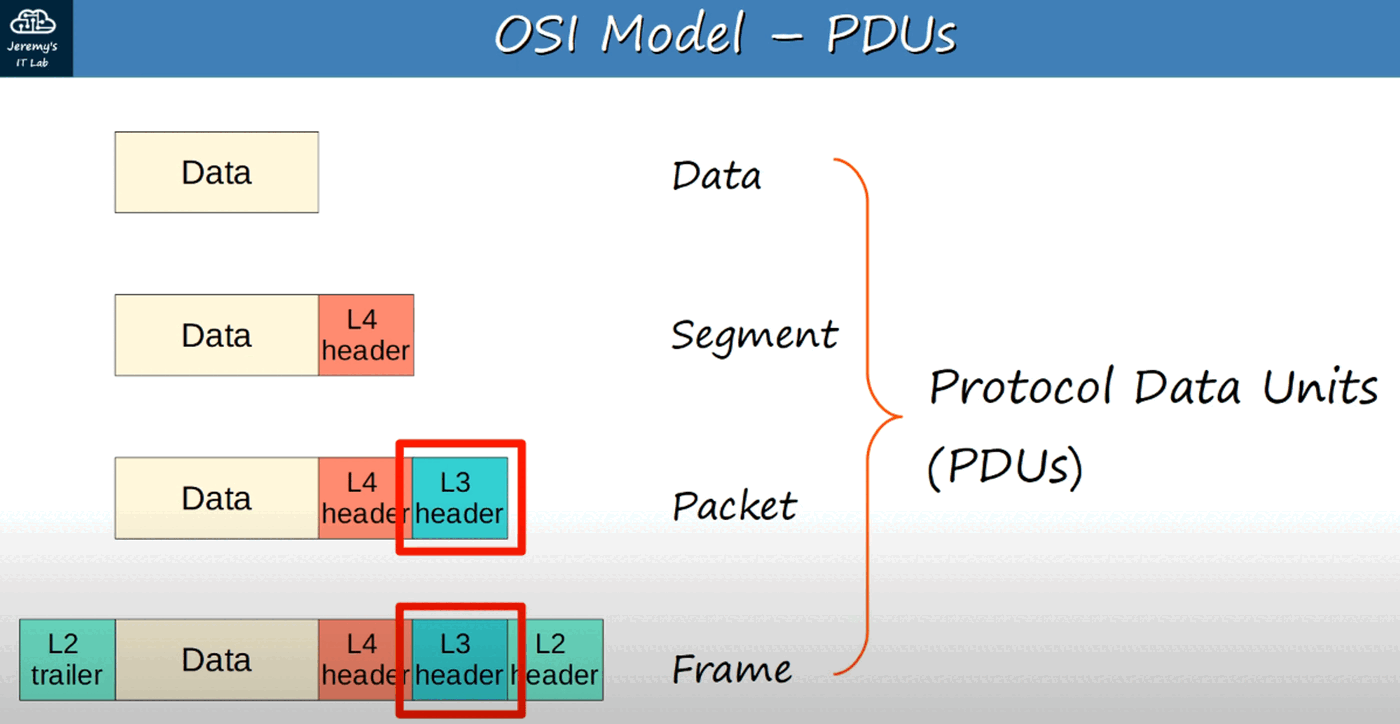
\includegraphics[keepaspectratio,alt={image}]{images/10-the-ipv4-header/img-001.png}}
\end{figure}

FIELDS OF THE IPv4 HEADER

\begin{figure}
\centering
\pandocbounded{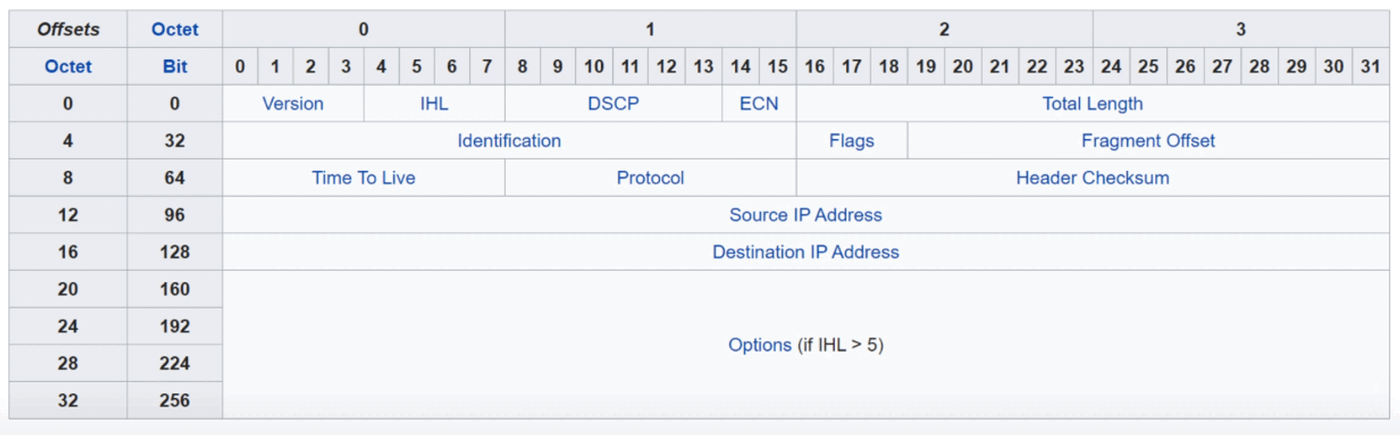
\includegraphics[keepaspectratio,alt={image}]{images/10-the-ipv4-header/img-002.png}}
\end{figure}

{\def\LTcaptype{none} % do not increment counter
\begin{longtable}[]{@{}ll@{}}
\toprule\noalign{}
FIELD & \# OF BITS \\
\midrule\noalign{}
\endhead
\bottomrule\noalign{}
\endlastfoot
VERSION & 4 \\
IHL & 4 \\
DSCP & 6 \\
ECN & 2 \\
TOTAL LENGTH & 16 \\
IDENTIFICATION & 16 \\
FLAGS & 3 \\
FRAGMENT OFFSET & 13 \\
TIME TO LIVE & 8 \\
PROTOCOL & 8 \\
HEADER CHECKSUM & 16 \\
SOURCE ADDRESS & 32 \\
DESTINATION ADDRESS & 32 \\
OPTIONS & 320 Max \\
\end{longtable}
}

\section{Version}\label{version}

\begin{itemize}
\tightlist
\item
  LENGTH is 4 bits.
\item
  IDs version of IP used (IPv4 or IPv6)

  \begin{itemize}
  \tightlist
  \item
    IPv4 = 0100 in Binary (Decimal 4)
  \item
    IPv6 = 0110 in Binary (Decimal 6)
  \end{itemize}
\end{itemize}

\section{Internet Header Length (IHL)}\label{internet-header-length-ihl}

\begin{itemize}
\tightlist
\item
  LENGTH is 4 bits.
\item
  Final field of IPv4 Header (Options) is variable in length so this
  field is necessary to indicate the total length of the header.
\item
  IDs the length of the header in 4-BYTE INCREMENTS.
\item
  The MINIMUM value is 5 (5 * 4-bytes = 20 bytes) - Empty OPTIONS Field
\item
  The MAXIMUM value is 15 (15 * 4-bytes = 60 bytes)
\end{itemize}

MINIMUM IPv4 HEADER LENGTH = 20 Bytes! MAXIMUM IPv4 HEADER LENGTH = 60
Bytes!

DSCP (Differentiated Services Code Point):

\begin{itemize}
\tightlist
\item
  LENGTH is 6 bits.
\item
  Used for QoS (Quality of Service)
\item
  Used to prioritize delay-sensitive data (streaming voice, video, etc.)
\end{itemize}

ECN (Explicit Congestion Notification):

\begin{itemize}
\tightlist
\item
  LENGTH is 2 bits.
\item
  Provides end-to-end (between two endpoints) notification of network
  congestion WITHOUT dropping packets.
\item
  Optional feature that requires both endpoints, as well as the
  underlying network infrastructure to support it.
\end{itemize}

\section{Total Length}\label{total-length}

\begin{itemize}
\tightlist
\item
  LENGTH is 16 bits.
\item
  Indicates the TOTAL length of the packet (L3 Header + L4 Segment)
\item
  Measured in bytes (not 4-byte increments like IHL)
\item
  Minimum value of 20 Bytes (IPv4 Header with NO encapsulated data)
\item
  Maximum value of 65,535 (MAXIMUM 16-bit value) = 2\^{}16
\end{itemize}

\section{Identification}\label{identification}

\begin{itemize}
\tightlist
\item
  LENGTH is 16 bits.
\item
  If a packet is fragmented due to being too large, this field is used
  to identify which packet the fragment belongs to.
\item
  All fragments of the same packet will have their own IPv4 header with
  the same value in this field.
\item
  Packets are fragmented, if larger than the MTU (Maximum Transmission
  Unit)
\item
  The MTU is usually 1500 bytes (Max size of an Ethernet frame)
\item
  Fragments are reassembled by the receiving host.
\end{itemize}

\section{Flags}\label{flags}

\begin{itemize}
\tightlist
\item
  LENGTH is 3 bits
\item
  Used to control/identify fragments.
\item
  Bit 0: Reserved, always set to 0.
\item
  Bit 1: Don't Fragment (DF bit), used to indicate a packet that should
  not be fragmented.
\item
  Bit 2: More Fragments (MF bit), set to 1 if there are more fragments
  in the packet, set to 0 for the last fragment or NO fragments.
\end{itemize}

\section{Fragment Offset}\label{fragment-offset}

\begin{itemize}
\tightlist
\item
  LENGTH is 13 bits
\item
  Used to indicated the position of the fragment within the original,
  unfragmented IP Packet.
\item
  Allows fragmented packets to be reassembled even if the fragments
  arrive out of order.
\end{itemize}

\section{Time to Live (TTL)}\label{time-to-live-ttl}

\begin{itemize}
\tightlist
\item
  LENGTH is 8 bits
\item
  A router will drop a packet with a TTL of 0
\item
  Used to prevent infinite loops
\item
  Originally designed to indicated a packets maximum lifetime in
  seconds.
\item
  In practice, indicates a `hop count': each time the packet arrives at
  a router, the router decreases the TTL by 1.
\item
  Recommended default TTL is 64.
\end{itemize}

\section{Protocol}\label{protocol}

\begin{itemize}
\tightlist
\item
  LENGTH is 8 bits
\item
  Indicates the protocol of the encapsulated Layer 4 PDU
\item
  Value of 1 : ICMP
\item
  Value of 6 : TCP
\item
  Value of 17 : UDP
\item
  Value of 89 : OSPF (Dynamic Routing Protocol)
\item
  List of protocol numbers on Wikipedia : List of IP Protocol Numbers
\end{itemize}

\section{Header Checksum}\label{header-checksum}

\begin{itemize}
\tightlist
\item
  LENGTH is 16 bits
\item
  A calculated checksum used to check for errors in the IPv4 header.
\item
  When a router receives a packet, it calculates the checksum of the
  header and compares it to the one in this field of a header.
\item
  If they do not match, the router drops the packet.
\item
  Used to check for ERRORS only in the IPv4 Header.
\item
  IP relies on the encapsulated protocol to detect errors in the
  encapsulated data.
\item
  Both TCP and UDP have their own checksum fields to detect errors in
  the encapsulated data.
\end{itemize}

SOURCE and DESTINATION:

\begin{itemize}
\tightlist
\item
  LENGTH is 32 bits each
\item
  SOURCE IP = IPv4 ADDRESS of the Sender of the Packet.
\item
  DESTINATION IP = IPv4 ADDRESS of the intended Receiver of the Packet.
\end{itemize}

\section{Options}\label{options}

\begin{itemize}
\tightlist
\item
  LENGTH is 0-320 bits
\item
  Optional / Rarely Used
\item
  If the IHL field is greater than 5, it means that Options are present.
\end{itemize}
